\documentclass[10pt,a4paper]{article}
\usepackage[latin1]{inputenc}
\usepackage{amsmath}
\usepackage{amsfonts}
\usepackage{amssymb}
\usepackage{color}
\usepackage{graphicx}
\usepackage{hyperref}
\usepackage{enumitem}
\usepackage{graphicx}
\hypersetup{
	colorlinks=true,
	linkcolor=blue,
	filecolor=magenta,
	urlcolor=cyan,
}
\RequirePackage[left=01.1cm,top=3cm,right=1.5cm,bottom=2.5cm,nohead,nofoot]{geometry}

\author{\vspace{0.4cm}
	Anirudh N J \\\vspace{0.4cm}
	Somesh Dev \\\vspace{0.8cm}
	Raina Thomas}

\title{
	\vspace*{5cm}
	\textbf{Scientific Experimentation and Evaluation}
	}
	
			
\begin{document}
	
\begin{titlepage}

	\maketitle
	
\end{titlepage}

\Large\textbf{PART I}	

\Large
\begin{enumerate}[label=\Roman*]
	\item
	\Large{\textbf{Aim}}\\
	
	Associate the terms given in the description of the soft tissue measurement experiment with appropriate terms from the slide "2B: Formalization general terms".
	\vspace{0.3cm}
	\item
	\Large{\textbf{Description}}\\
	
	\begin{itemize}
		\item	
		\textbf{Measurand :}
		\begin{itemize}
			\item
			Force in the axial direction
		\end{itemize}
		
		\item
		\textbf{Measurement :}
		\begin{itemize}
			\item
			Torque(N)
		\end{itemize}
		\item
		\textbf{Measuring Principle :}
		\begin{itemize}
			\item
			Strain Gauge
		\end{itemize} 
		\item
		\textbf{Measurement facility :}
		\begin{itemize}
			\item
			PI hexapod
			\item
			Monocarrier drive
			\item
			Indentation tool
			\item
			Simulab complex tissue model
			\item
			ATI Mini40 force sensor
			\item
			EPOS2 motor controller
		\end{itemize} 
		\item
		\textbf{Device Under Test (DUT):}
		\begin{itemize}
			\item
			Tissue Analogue
		\end{itemize} 
		\item
		\textbf{Sensitivity :}
		\begin{itemize}
			\item
			Axial force resolution of 0.04N
		\end{itemize} 
		\item
		\textbf{Measurement System :}
		\begin{itemize}
			\item
			EPOS2 motor controller
			\item
			Indentation tool
			\item
			FT sensor
			\item
			NI DAQ
		\end{itemize}
		\item
		\textbf{Meter :}
		\begin{itemize}
			\item
			FT sensor
			\item
			NI DAQ
		\end{itemize}
		\item
		\textbf{Measuring method: }
		\begin{itemize}
			\item
			Displace the material using the indentation tool.
			\item
			Measure the applied force using FT sensor.
		\end{itemize}
		
		
		
	\end{itemize}
	
	
\end{enumerate}	
\newpage
\Large\textbf{PART II}

\Large
\begin{enumerate}[label=\Roman*]

\item
\vspace{0.5cm}
\Large{\textbf{Aim}}\\

The aim of this project is to construct a LEGO NXT differential drive robot and measure the observable end pose variation for three different trajectories: an arc to the left, driving straight and an arc to the right.
\vspace{0.5cm}

The experiment of measuring the end pose can be done in three ways :
\begin{enumerate}
    \item
    Measuring the pose manually using a pen
    \item
    Measuring the pose using a pen attached to the robot
    \item
    Measuring the pose using markers and Computer Vision 
\end{enumerate}    

\vspace{0.5cm}
\item
\Large{\textbf{Experimental Setup}}\\
\vspace{0.5cm}

To reproduce the above experiment the following equipment are needed :
\begin{enumerate}
    \item
    White A1 Sheet
    \item
    Camera - Microsoft 
    \item
    Assembled robot - Lego NXT 
    \item
    Pens for marking
    \item
    Scales for measuring the length 
    \item
    Vision markers
\end{enumerate}
\vspace{0.5cm}

The general steps to setup the experiment are as following :
\begin{enumerate}
    \item
    Place the White A1 sheet on a flat surface.  Try to remove any bends in the sheet and keep the paper as flat as possible. This will be called the 'map' on which the robot will move on. The measurement system is made of the robot, scale and a paper. 
    \item
    Mark the center of the A1 sheet using the scale and a pencil.
    \item
    Draw the template drawing of the "floor space" taken by the robot as shown in the figure. Concept of "Behavior-shaping constraint" is used to prevent wrong initial placement of the robot.
    
    
    \begin{figure}[h]
	\centering
    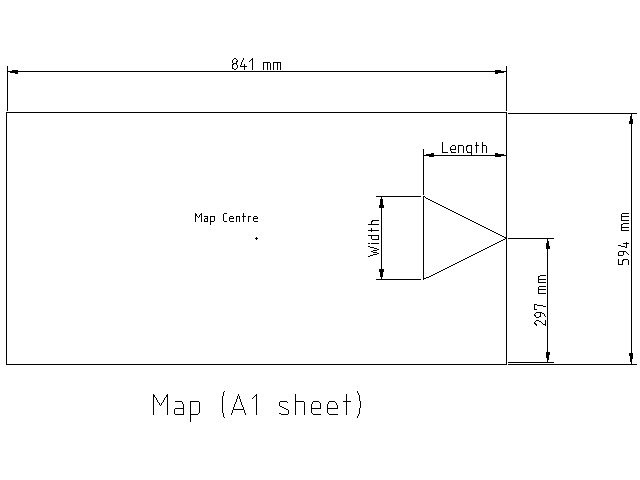
\includegraphics[width=0.6\linewidth ]{Template.png}
    \caption{ Template drawing of the Map along with dimensions}
    \end{figure}

    \item
    Assemble the robot using the manual given with the LEGO NXT box. Install the OS to the controller of the robot. The Lego robot is the device under test(DUT). 
    \item
    We assume that the driving axle is towards the front(leading edge) of the robot and that the robot origin lies in the centre of the driving axle.
    \item
    Place the robot such that the centre of the robot aligns with the centre of the A1 sheet on one of its shorter edges.
    \item
	The measurands are the distance between the initial and end positions and the angles between the two poses.
    
\end{enumerate}
\vspace{0.5cm}

The reference images of the DUT and the proposed marker tracking visualization are given below.

\begin{figure}[h]
	\centering
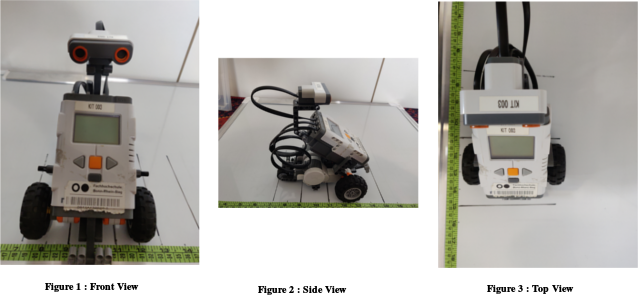
\includegraphics[width=0.8\linewidth ]{pose.png}
\caption{ Views of the DUT- with approximate dimensions}
\end{figure}

\vspace{0.5cm}
\item
\Large{\textbf{Experimental Procedure}}\\

\begin{enumerate}[label=\roman*)]

\item 
\Large{\textbf{Measuring the pose manually using a pen}}\\

\begin{enumerate}

\item
\Large{\textbf{Procedure}}\\

\begin{enumerate}
	\item
	The measurement system is made of the robot, scale and a paper. The scale is used to measure the distance of the end pose of the robot relative to the start pose. 
	\item
	The robot pose is measured using two markings, one on the centre of the leading edge of the robot and another on the centre of the trailing edge of the robot. 
	\item
	The initial pose of the robot is manually marked at the beginning using the pen.
	\item
	The robot is programmed to move using the initial pose and the desired final pose.
	\item
	The distance between the initial and final poses and the angles between the initial and the final poses are calculated using the front and the rear markings. These values can be used to calculate the pose.
	\item
	20 measurements would be performed for each trajectory. Mean and standard deviation will be computed from the measurement. These measured values would be used to compute the accuracy and precision of the pose variation. 
\end{enumerate}
\vspace{0.5cm}

\item
\textbf{Expected Problems}\\
\begin{enumerate}
	\item
	There can be errors due to wheel slip which are negligible if the distance travelled by the robot is less.
	\item
	Manual error may occur when marking the pose of the robot using a pen.
	\item 
	Parallax error may occur when a marking is made manually using the pen.
	\item
	The robot should not move when the marking is made or it can lead to drawing inconsistent pose markings. 
	\item
	Uneven surface of the paper could cause change in trajectory.
\end{enumerate}
\vspace{0.5cm}

\item
\textbf{Expected Performance}\\
\begin{enumerate}
	\item
	The precision would not be perfect, but could have a large range since the DUT and the measurement facility are all manual and may involve errors due to direct contact with the apparatus.
	\item
	The accuracy depends strongly on the problems listed for the experiments. The most important problems would be the error due to manual marking where the chances of the contact with the robot are very high. Since the distance driven is maximum 1m, the error in precision and accuracy will lie in the centimeter range.
\end{enumerate}
\end{enumerate}
\vspace{0.5cm}

\item 
\Large{\textbf{ Measuring the pose using a pen attached to the robot}}\\

\begin{enumerate}

\item
\Large{\textbf{Procedure}}\\

\begin{enumerate}
	\item
	The Lego robot, which is the device under test(DUT), is built with a pen mounted in the front, back or the center of the robot.
	\item
	The measurement system is made of the robot, scale and a paper. The scale is used to measure the end pose of the robot relative to the start pose. The path taken by the robot is sketched on the paper by the pen.
	\item
	The initial pose of the robot is manually marked at the beginning along with the alignment of the wheels to measure the angular displacement at the final pose.
	\item
	The robot is programmed to move using the initial pose and the desired final pose.
	\item
	The measurands are the distance between the initial and end positions and the angles between the two poses.
	\item
	20 measurements would be performed for each trajectory. Mean and standard deviation will be computed from the measurement. These measured values would be used to compute the accuracy and precision of the pose variation. 
\end{enumerate}
\vspace{0.5cm}

\item
\textbf{Expected Problems}\\
\begin{enumerate}
    \item
    Errors such as wheel slip and internal errors in the robot drive can cause errors in the final calculation.
	\item
	The errors in measurement if the A1 sheet is not properly placed is very difficult to measure.
	\item
	The pen can wobble and affect the shape of the curve and thereby the result.
	\item
	Uneven surface of the paper could cause change in trajectory.
\end{enumerate}
\vspace{0.5cm}

\item
\textbf{Expected Performance}\\
\begin{enumerate}
	\item
	The precision would not be perfect, but could have a small range since the DUT and the measurement facility are not changed.
	\item
	There is minimum manual intervention during the actual pose measurement so the major contributor of error will be due to the movement of the pen when the robot is moving. 
	\item
	The accuracy depends strongly on the problems listed above. The most important problems would be the error due to wheel slip. Since the distance driven is maximum 1m, the error in precision and accuracy will lie in the centimeter range.
	
\end{enumerate}
\end{enumerate}
\vspace{0.5cm}


\item 
\Large{\textbf{ Measuring the pose using markers and Computer Vision}}\\

\begin{enumerate}

\item
\Large{\textbf{Procedure}}\\

\begin{enumerate}
	\item
	For this experiment the camera should be placed rigidly directly above the experiment setup such that the full map is visible in the camera frame. 
	\item
	Before beginning the experiment the camera should be calibrated and the obtained parameters should be used to compensate for the lens distortion and other errors in the image. 
	\item
	Two small markers should be attached on the flat surface of the robot, one on the front and one on the rear of the robot. The markers should be visible in the camera frame captured by the overhead camera. (The two markers should have different ID to distinguish between them)
	\item
    Using Computer-vision the two markers on the robot can be tracked and localized. The centre of the markers can be found and be used to calculate the offset from the actual robot origin using a scale or any other measuring device.
	\item
	The robot is programmed to move using the initial pose and the desired final pose.
	\item
	The initial pose and the final pose can be found by CV and position and pose in the required form can be extracted.
	\item
	20 measurements would be performed for each trajectory. Mean and standard deviation will be computed from the measurement. These measured values would be used to compute the accuracy and precision of the pose variation. 
\end{enumerate}
\vspace{0.5cm}

\begin{figure}[h]
	\centering

\includegraphics[width=0.2\linewidth ]{marker.png}
\caption{ Example Aruco marker for computer vision}
\end{figure}

\item
\textbf{Expected Problems}\\
\begin{enumerate}
	\item
	There could be problems due to the setup not done correctly. eg. The paper is not perfectly flat.
	\item
	Camera is not fixed rigidly enough.
	\item
	Camera calibration is not performed correctly.
	\item
	Software related bugs in the logic of the computer vision code.
\end{enumerate}
\vspace{0.5cm}

\item
\textbf{Expected Performance}\\
\begin{enumerate}
	\item
	This experiment accuracy and precision depends highly on the setting up of the camera and the markers correctly.
	\item
	Since the experiment does not rely on any manual intervention or has no moving parts like the pen, the precision is very high.
\end{enumerate}
\end{enumerate}
\vspace{0.5cm}


\end{enumerate}


	

\end{enumerate}	






\end{document}


